\documentclass[
    a4paper,
    man,
    floatsintext,
    british
]{apa6}

\usepackage{booktabs}
\usepackage[british]{babel}
\usepackage[utf8]{inputenc}
\usepackage{epstopdf}
\usepackage{csquotes}
\usepackage[hidelinks]{hyperref}
\usepackage[
    style=apa,
    backend=biber,
    sortcites=true,
    sorting=nyt,
%    isbn=false,
%    url=false,
%    doi=false,
%    eprint=false,
    hyperref=false,
    backref=false,
%    firstinits=false,
]{biblatex}

\DeclareLanguageMapping{british}{british-apa}

% maps apacite commands to biblatex commands
\let \citeNP \cite
\let \citeA \textcite
\let \cite \parencite

%%%
% Apa Bib - enable reprint according to apa
%%%

% http://tex.stackexchange.com/questions/139805/how-to-differentiate-between-translated-and-reprinted-work-with-apa-style

\renewbibmacro*{related:reprintfrom}[1]{%
  \entrydata*{#1}{%
    \printtext{\mkbibemph{\printfield[apacase]{title}}}%
    \setunit{\bibpagespunct}%
    \printfield{pages}%
    \setunit{\addcomma\addspace}%
    \bibstring{byauthor}\addspace
    \printnames[apanames][-\value{listtotal}]{editor}%
    \ifnameundef{editor}
      {}
      {\addcomma\addspace
       \usebibmacro{apaeditorstrg}{editor}}
    \printnames[apanames][-\value{listtotal}]{author}%
    \setunit{\addcomma\addspace}%
    \usebibmacro{date}%
    \setunit{\addcomma\addspace}%
    \usebibmacro{location+publisher}%
    \newunit\newblock
    \usebibmacro{related}}}


\DefineBibliographyStrings{british}{
  reprintfrom = {Reprinted from}
}


\bibliography{Thesis1}


%%%%%%%%%%%%%%%%%%%%%%%%%%%%%%%%%%%%%%%%%%%%%%%%%%%

\title{Effects of Offloading on Visual Working Memory: A Behavioural Study}
\shorttitle{Offloading in Visual Working Memory}
\author{Anushree Ganesh}
\affiliation{Utrecht University}



\begin{document}

\maketitle
\section{Abstract}
An incessant amount of visual information is accrued in our working memory on a day-to-day basis. To maintain the efficiency of cognitive processes, there must be a mechanism by which irrelevant information is dropped or offloaded from the visual working memory. This study aims to understand if items that no longer need storing as they are (again) available externally can be offloaded and if offloading affects visual working memory. It aims to bridge the knowledge gap caused by the limited literature on offloading in visual working memory. This behavioural experiment reports on the differences in median response times and sensitivities across different offloading conditions compared to the baseline condition. A convenience sample of 28 participants aged between 18 to 26 years participated in this experiment. Results showed that response times were faster across the different offloading conditions than the baseline condition. Further, the d-prime analysis revealed that the participants performed slightly better than the chance level and likely found the task too hard. In conclusion, the results indicated promising effects of offloading on visual working memory.

\section{Introduction}
Working memory is a vital component of human memory and temporarily holds cognitive representations used in thought and action \parencite{oberauer_2018_removal}. A key aspect of working memory is visual working memory, where limited visual information is stored and manipulated through attentional networks \parencite{gao_2016_objectbased}. We are exposed to extensive amounts of visual information in our environment concurrently. Due to the limited working memory capacity, a mechanism must be employed to constantly update relevant information and remove irrelevant information \parencite{lewispeacock_2018_the}. Visual representations of the external world are imprecise and severely limited \parencite{ramosgameiro_2017_exploration}. If there is visual information available in the external world, then items are not stored in the working memory as the external world serves as a memory source \parencite{ballard_1995_memory, somai_2020_evidence}. Conversely, if items are stored in the visual working memory, and if the information is made available again in the external environment, can items stored in the visual working memory be dropped? This was the primary motivation behind the study, which led to the main question – can irrelevant information be offloaded from memory if it becomes available again in the environment?
\\
In previous studies, the term ‘offloading’ or ‘cognitive offloading’ has been used to describe the process of reducing mental efforts during a task through physical actions, such as taking notes \parencite{morrison_2020_offloading}. Throughout this study, offloading will refer to the process by which items are removed or dropped from visual working memory. A growing body of literature has investigated offloading in working memory differently \parencite{dames_2022_, lintz_2021_refreshing, oberauer_2018_removal, shan_2022_the, vergauwe_2014_the}. However, there is limited literature on offloading in visual working memory. 
\\
This thesis intends to bridge this knowledge gap. More specifically, it aims to answer how the information in the environment affects what is dropped from our memory and what is not. To this end, the main research question was - How does the possibility of offloading items from visual working memory as they become re-available in the external world affect task performance (i.e., accuracy and speed)?
\\
Data were collected from a convenience sample. The experimental design consisted of four conditions, three offloading and one baseline condition. Participants were tasked with recalling feature-based stimuli. The stimuli were adapted and used from \textcite{endo_2003_perceptual}. A set of 4 stimuli were presented on the screen for 300 ms (encoding period) to be memorised, after which a blank retention screen was presented for 500 ms. Then, either 1,2 or 3 of the non-target stimuli were randomly selected and re-presented (offloading condition), or no stimuli were re-presented (baseline condition). The participants were either shown a random non-target or the target stimulus as a probe image and were asked to respond with a ‘yes’ if it was a part of the stimulus set presented or ‘no’ if it was not. 
\\
The current study investigated the effects of offloading by comparing the median response times across the different offloading conditions and the baseline condition. The main hypotheses were as follows:
\begin{enumerate}
  \item Hypothesis 1: There would be a significant difference in median response times between offloading and baseline conditions. It was a two-sided hypothesis.
  \item Hypothesis 2: There would be a significant difference in the sensitivities (d-prime analysis) between offloading and baseline conditions. 
\end{enumerate}
This work will give a fresh insight into the process of offloading in visual working memory. This thesis comprises the following four sections – methods, results, discussion, conclusion and prospects.

\section{Methods}

\subsection{Participants}
A convenience sample of students from Utrecht University participated in this experiment (\textit{n} = 28). Of the 28 participants, 22 identified as female (78.5\%), four as male (14.2\%), and two as non-binary (7.1\%). The participants’ age ranged from 18 to 26 years (\textit{M} = 20.75, \textit{SD} = 1.97). All but four participants were right-handed. No psychiatric, neurological, or ophthalmological conditions were reported. All participants gave written informed consent. The participants were naïve about the hypothesis. All statistical tests reported were two-sided.

\subsection{Stimuli and Apparatus}
The experiment was presented on a standard Windows 10 PC via a 23-inch monitor. The screen resolution was 1920$\times$1080 pixels with a 60 Hz refresh rate. The experiment was built and presented on PsychoPy (v2021.2.3). A chinrest was used to standardise the distance from the monitor for every participant and to ensure they faced the centre of the screen at all times. The monitor was positioned 63.5 cm away from the eye position. Feature-based stimuli were used to prevent verbalisation. They were 8.24°$\times$8.24° in width and height. All visual stimuli were presented on a white background. Responses were collected via two external keys, ‘y’ and ‘n’, corresponding to ‘yes’ and ‘no’ responses. 
\subsection{Procedure}
All participants were tested individually in a single 1-hour session. The sequence of trials is illustrated in Figure 1. The trial started with a blank screen with a fixation circle (500 ms), followed by the presentation of four randomly selected image stimuli (300 ms). A delay period (500 ms) then showed four blank boxes, after which zero, one, two or three non-target image stimuli were presented again (500 ms). A valid blue-coloured retrocue box in the position of the target stimuli was then presented. A probe image was presented on top of the boxes with either the target stimuli or another neutral stimulus (until response). 
\\
Participants were instructed to compare and recall whether the probe image presented at the end was present in the position of the retrocue box or not. If the probe image was present in the position of the retrocue box, then they would have to respond ‘yes’; if not, with ‘no’. Participants pressed the ‘y’ key with their left-hand index finger if the response was ‘yes’ and with their right-hand index finger if the response was ‘no’. 
\\
All participants performed all four conditions in this experiment. The baseline condition was condition 0, where zero images were shown after the delay period. The offloading conditions were - condition 1, where one randomly selected image was shown after the delay period; condition 2, where two randomly selected images were shown after the delay period; and condition 3, where three randomly selected images were shown after the delay. The conditions were evenly distributed over all 168 trials randomly (42 trials per condition). The first eight trials were practice trials, after which there was a short break. Participants also received a short break at the halfway point between trials. The experimenter stayed in the room to monitor compliance and answer any questions.

%task figure
\begin{figure}[hbt!]
    \centering
    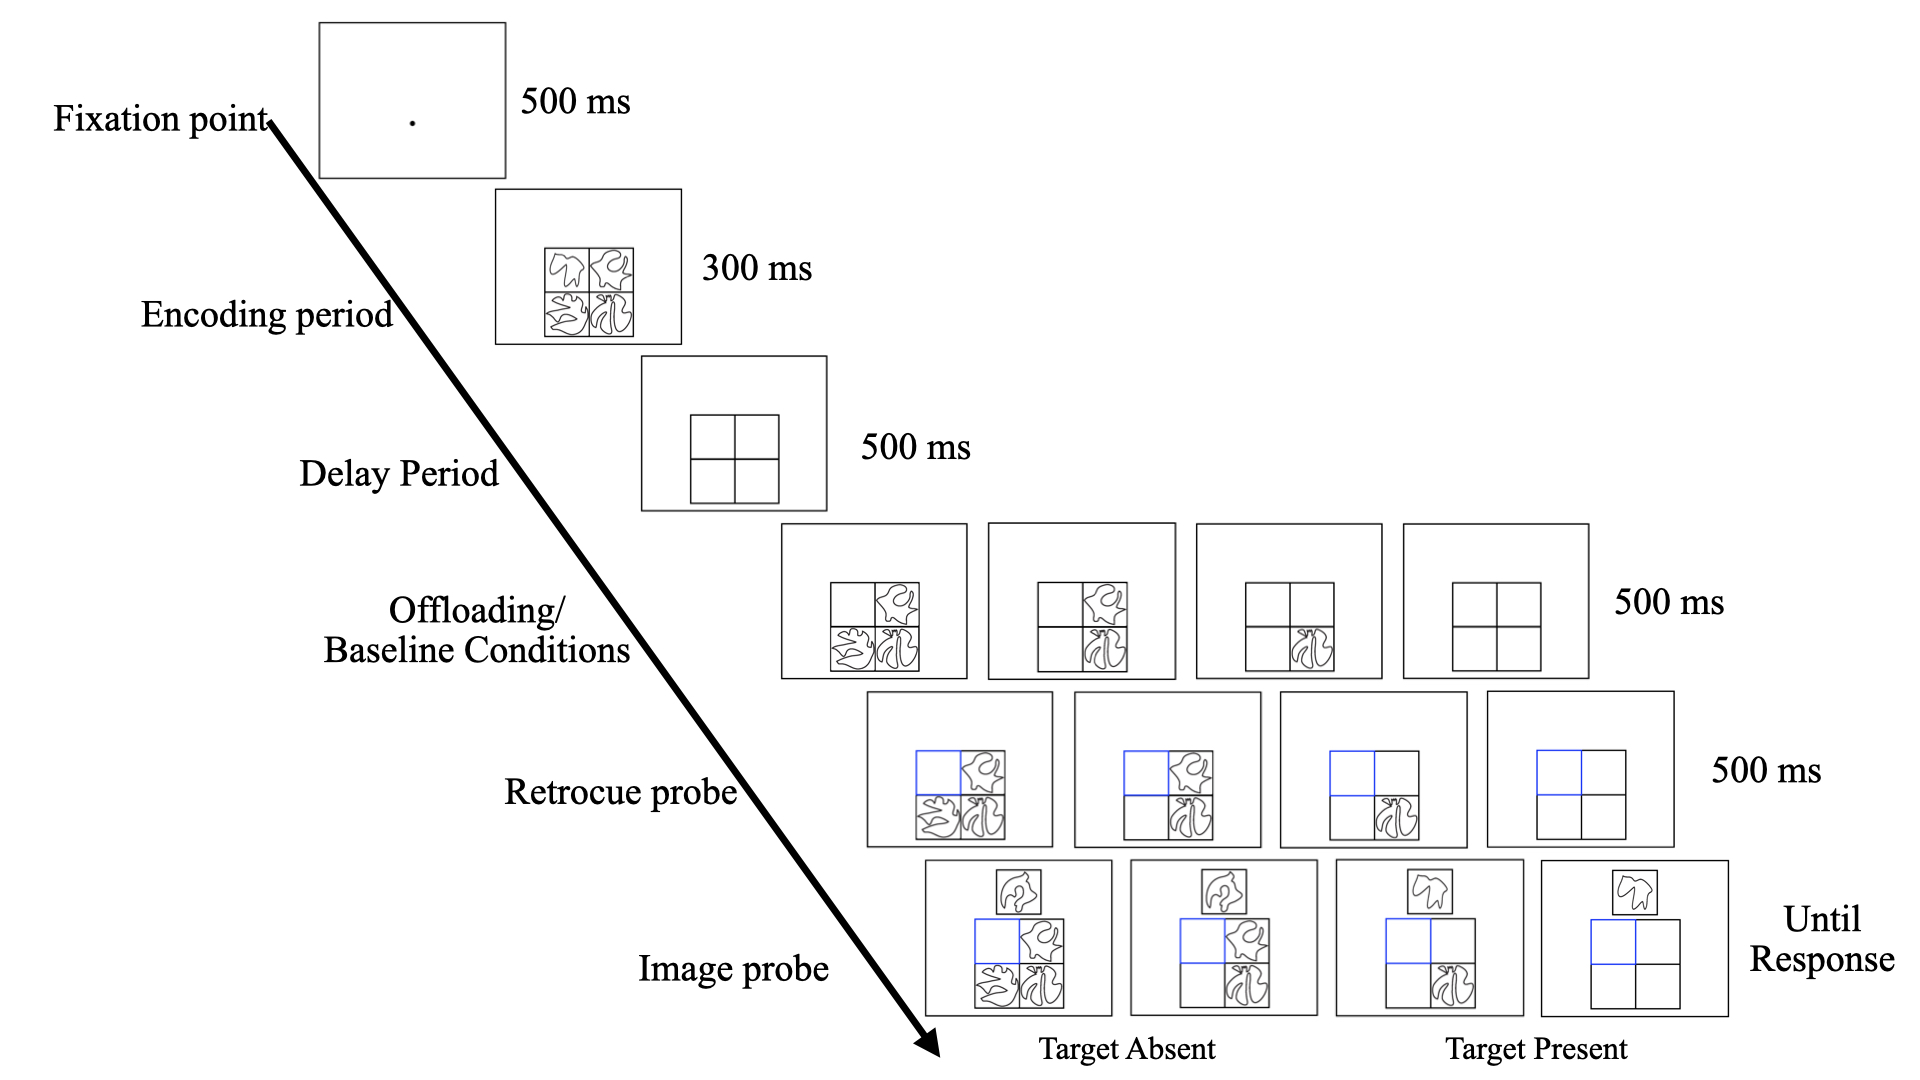
\includegraphics[scale = 0.24]{task figure.jpeg}
    \caption{Sequence of trial task figure. The trial began with a fixation circle (centred on the x-axis), and then four feature-based stimuli were presented to be memorised. Four blank boxes were presented during the delay period, after which images were presented according to one of the four conditions (0, 1, 2, or 3). A blue box was used as a retrocue, and participants compared the target stimuli with the probe image displayed on top (target present probe or target absent probe).}
    \label{fig:task_fig}
\end{figure}

\newpage
\subsection{Data processing and Analysis}
All data were processed using Python (3.10.8). Statistics were conducted using JASP (version 0.16.4). The four different conditions resulted in a repeated-measures ANOVA experimental design. The analysis focused on the difference in response times (RTs) per condition and the d-prime values per condition. The median correct and incorrect RTs per condition were also analysed. Participants with d-prime values close to 0 or -1 were excluded from the analysis as they indicated poor execution of the task. A significance level of $\alpha = .05$ is adopted. 

\newpage
\section{Results}
It was hypothesised that if dropping items from visual working memory is possible, then it would affect the response times and sensitivities (d-primes) of participants in the offloading conditions where offloading images were presented (1, 2, and 3) as compared to the baseline condition where no offloading images were present (0).
\\
A two-way repeated measures ANOVA determined that participants responded faster in the offloading conditions compared to the baseline condition, \textit{F}(3,75) = 20.18, \textit{p} <.001 (See Figure 2A). An ANOVA with correctness (correct responses, incorrect responses) and conditions (baseline - 0, offloaded - 1, 2, 3) as factors revealed the main effects for both the factors (condition, \textit{F}(3,75) = 13.62, \textit{p} <.001; correctness, \textit{F}(1,25) = 35.05, \textit{p} <.001) and an insignificant interaction (\textit{F}(3,75) = 1.94, \textit{p} = 0.131). This result supported hypothesis 1. It is illustrated in Figure 2B.


%medianRT figures
\begin{figure}[hbt!]
    \centering
    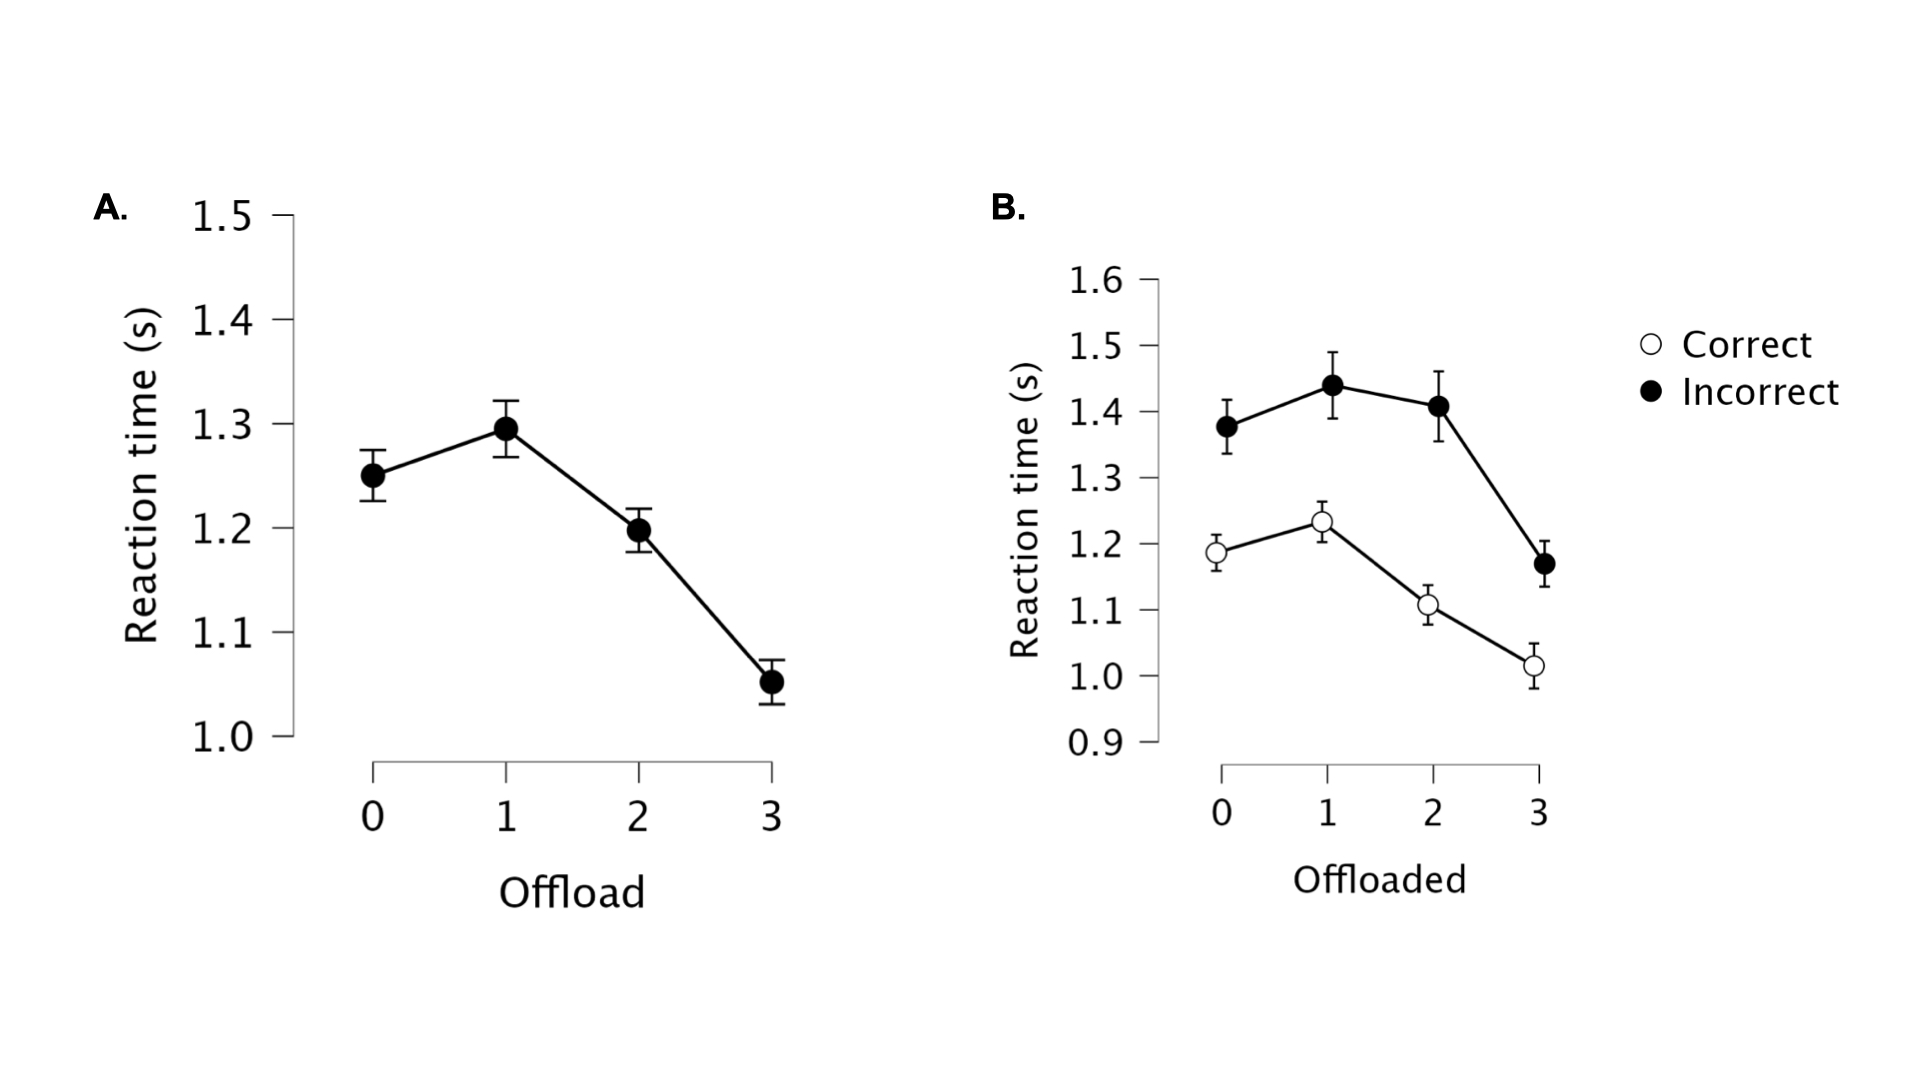
\includegraphics[scale = 0.2]{medianRT.jpeg}
    \caption{\textbf{A.} Shows the median reaction times averaged over all the participants for the three offloading conditions (1, 2, and 3) with respect to the baseline condition (0) where no offloading images were present. \textbf{B.} Visualises the median reaction times in correct and incorrect trials averaged over all the participants for the three offloading conditions (1, 2, and 3) with respect to the baseline condition (0) where no offloading images were present.}
    \label{fig:medianRT}
\end{figure}

\newpage
%Table1
\begin{table}[htb!]
	\centering
	\caption{Within Subjects Effects: Significant differences in the median response times of participants in the various offloading conditions}
	\label{tab:medianRT}
	{
		\begin{tabular}{lrrrrrr}
			\toprule
			Cases & Sum of Squares & df & Mean Square & F & p & $\eta_p^2$  \\
			\cmidrule[0.4pt]{1-7}
			Offload & $0.854$ & $3$ & $0.285$ & $1.032$ & $0.383$ & $0.040$  \\
			Residuals & $20.681$ & $75$ & $0.276$ &  &  &   \\
			\bottomrule
			% \addlinespace[1ex]
			%\multicolumn{7}{p{0.5\linewidth}}{\textit{Note.} Type III Sum of Squares} \\
		\end{tabular}
	}
\end{table}

\begin{table}[hbt!]
	\centering
	\caption{Within Subjects Effects: Significant differences in correctness and offloading factors in the median response times of participants}
	\label{tab:correctRT}
	{
		\begin{tabular}{p{3cm} p{1.5cm}p{0.75cm}p{2cm}p{1.5cm}p{1.5cm}p{1cm}p{1cm}}
			\toprule
			Cases & SS & df & Mean Square & F & p & $\eta^2$ & $\eta_p^2$  \\
			\cmidrule[0.2pt]{1-8}
			Offloaded & $1.722$ & $3$ & $0.574$ & $13.628$ & $<$ .001 & $0.156$ & $0.353$  \\
			Residuals & $3.159$ & $75$ & $0.042$ &  &  &  &  \\
			Correctness & $2.359$ & $1$ & $2.359$ & $35.058$ & $<$ .001 & $0.214$ & $0.584$  \\
			Residuals & $1.682$ & $25$ & $0.067$ &  &  &  &   \\
			Effect & $0.150$ & $3$ & $0.050$ & $1.935$ & $0.131$ & $0.014$ & $0.072$  \\
			Residuals & $1.941$ & $75$ & $0.026$ &  &  &  &  \\
			\bottomrule
			 \addlinespace[1ex]
			\multicolumn{8}{p{1\linewidth}}{\textit{Note.} SS = Sum of Squares and Effect = Offloaded * Correctness} \\
		\end{tabular}
	}
\end{table}

In order to analyse how well the participants executed the task, signal detection theory was used. To this end, d-prime is computed based on the z-scores of hit rates and false alarm rates. A two-way repeated measures ANOVA determined that the average d-prime did not significantly differ in the offloading conditions compared to the baseline condition, \textit{F}(3,75) = 1.03, \textit{p} = 0.38 (See Figure 3). The participants did not execute the task differently across the four conditions. Most participants performed slightly better than the chance level and might have found the task too complicated(\textit{$M_{d'}$}= 0.84,\textit{SD} = 0.56). This result did not support hypothesis 2.
%dprime figure
\begin{figure}[hbt!]
    \centering
    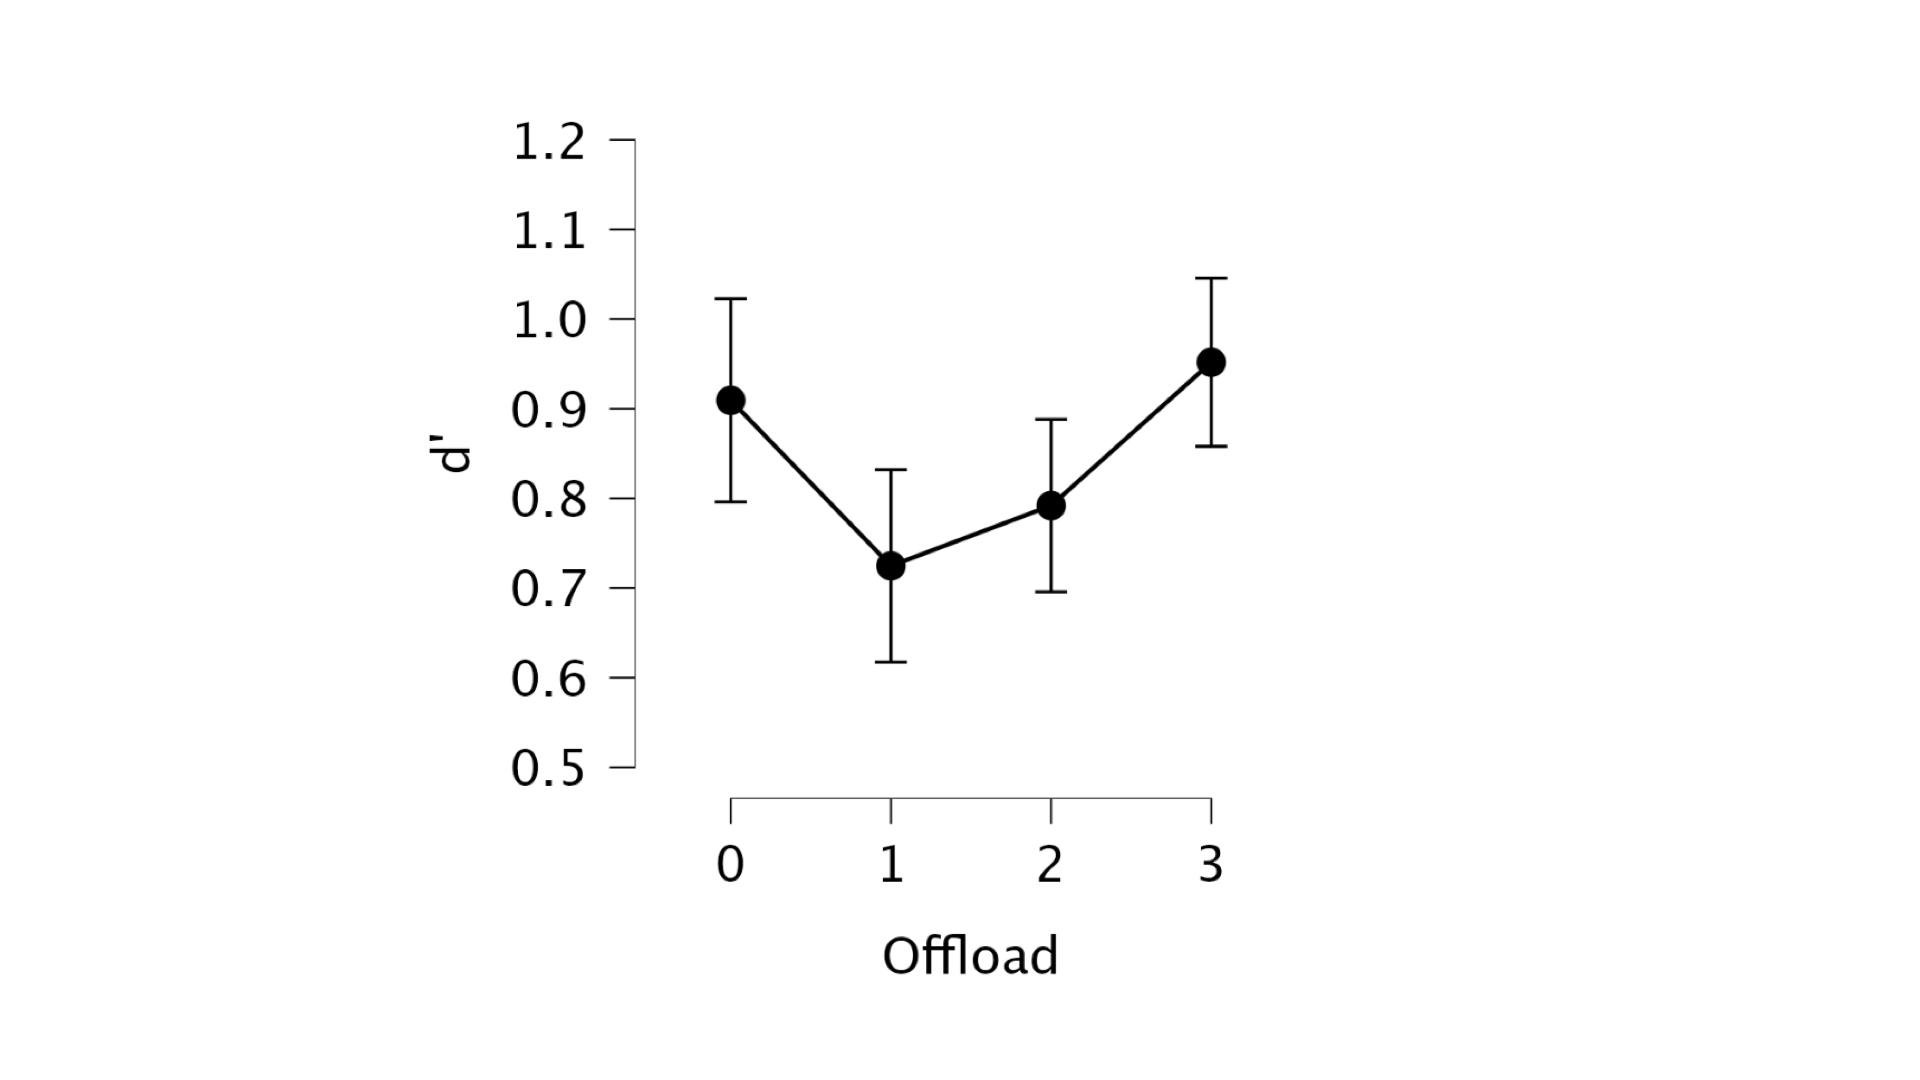
\includegraphics[scale = 0.2]{dprime.jpeg}
    \caption{Shows the average \textit{$d'$} for each of the three offloading conditions (1, 2, and 3) with respect to the baseline condition (0) of all the participants.}
    \label{fig:dprime}
\end{figure}

\newpage
\section{Discussion}
The present study was designed to determine whether items can be dropped or offloaded from memory and whether offloading has an effect on visual working memory. To this end, a retrocue visual memory recall task was built. The parameters consisted of an encoding period of 300 ms, a delay period of 500 ms and a probe onset of 500 ms. The task tested three offloading conditions and one baseline condition, and the response times for each trial were recorded. The results indicated that there were significant differences in response times which were observed in the offloading conditions compared to the baseline condition. Consequently, the d-prime analysis concluded that most participants were at chance level regarding the execution of the task. 
\\
The different offloading conditions have varying degrees of complexity. For instance, in the least complex condition, i.e. condition 3, the participant had to draw a comparison with just one missing box and one probe image. In contrast, in the most complex condition, i.e. condition 1, the participant had to draw a comparison with three missing boxes and one probe image. An increase in perceptual complexity increases the information load, resulting in longer response times \parencite{eng_2005_visual, onken_1985_individual}. The varying complexity of decision-making could explain the substantial differences in the response times for the different conditions. 
\\
On the contrary, the d-prime analysis showed that participants were only slightly better than the chance level regarding the execution of the task. This is likely because the participants found the task to be complicated. A contributing reason could be that the encoding period (300 ms) was too short, which is also one of the weaknesses of this study. \textcite{janczyk_2014_orienting} propose that the encoding period should be at least 900 ms. They define anything under 900 ms to be encoded into iconic memory instead. \textcite{bays_2011_temporal} and \textcite{gao_2016_objectbased} concluded that more extended encoding periods of 500 ms to 1000 ms yielded accurate and faster responses compared to shorter encoding periods of 100 ms to 300 ms. Another limitation of the study was the complexity of the chosen stimuli. While it aimed at preventing verbalisation during memory recall, the perceptual complexity could have also hindered the ability to execute the task well \parencite{eng_2005_visual}. 
\\
Although it has been suggested that iconic memory encoding takes place below 900 ms, there is an intrinsic overlap between sensory components of iconic memory and visual working memory \parencite{bradley_2012_the}. They also suggest that this overlap, further compounded by individual variabilities, makes defining a generalisable hard limit challenging. This study raises the possibility of understanding the nature and extent of visual working memory and how it is organised. These observations have important implications for defining and developing mechanisms to offload irrelevant items from visual working memory. This study's results were encouraging and pointed to the many unanswered questions in the field.
\newpage
\section{Conclusion and Prospects}
The present study aimed to understand if offloading is possible and its effects on visual working memory. Median response times indicate that participants are significantly faster at responding during the offloading than the baseline conditions. The results thus suggest that offloading allowed participants to speed up their response times, however, the sensitivity of their responses did not change. Some of the study's limitations included the short encoding period (300 ms) and the complex stimuli used in this study.
\\
A further study could assess offloading using more extended encoding periods, around 500 ms to 1000 ms. Future research can also utilise simpler stimuli to overcome the hindrances experienced by the participants in the present study. A natural progression of this work would be to analyse the offloading process through pupillometry or EEG. These methods could give insight into the mental efforts that participants put in during offloading and could observe whether offloading impairs or improves visual working memory.  
\\
Taken together, the findings in this study imply some promising effects of offloading, as seen by the differences in response times. Future studies could tackle the potential benefits of accuracy and sensitivity of the task, for instance, by making the task easier and validate the present study's effects in further detail.
\newpage
\printbibliography
\newpage
\section{Acknowledgements}
I would like to start by thanking my family - my parents, and my brother for always supporting me in all my endeavours. I would like to thank Vidya Mami, Shiva Mama and Nidhi, for being my second home. Manya, thank you for always being there to remind me of the warmth of our friendship, and to breathe easy during trying times.
\newline
\\
I would also really like to thank my supervisor, Christoph, for encouraging me to focus on learning throughout the course of this Thesis. And thank you Damian, for all the patience you have exhibited throughout and especially while we were fighting off silly strings in code. I have learnt, felt challenged, and had more fun along the way than I could have ever imagined. Thank you both for always being there to answer my questions and for guiding me through my first steps in research.
\newline
\\
Desai, I cannot begin to thank you for lending so much of your mindful patience, understanding and for believing in me always, but especially when I could not. Thank you for inspiring me to work hard consistently and for teaching me how to code. But thank you the most for being my best friend. 
\newline
\\
\textbf{Lastly, I dedicate this Thesis to my uncle, Narayan Mama, who was my biggest cheerleader.}

\end{document}
